\documentclass[border=1.5pt]{standalone}
\usepackage{amsmath,amssymb}
\usepackage{tikz}
\usetikzlibrary{arrows.meta,calc,positioning,shapes,shapes.misc,shapes.geometric,backgrounds,fit,decorations.pathreplacing,quantikz2}
% Shared colors and styles for the XYZ^2 figures.
% Pauli types: bright tones for fills and bands, deep (800) shades of the same hues for labels.
% The label shades keep the hue of each Pauli, are well separated from each other (CIEDE2000 > 20)
% and have a contrast ratio of at least 2.9 on the coral cells and 4.5 on the sunflower cells.
\definecolor{PauliX}{HTML}{F97316}
\definecolor{PauliY}{HTML}{EC4899}
\definecolor{PauliZ}{HTML}{9333EA}
\definecolor{PauliXText}{HTML}{AC340B}
\definecolor{PauliYText}{HTML}{9D174D}
\definecolor{PauliZText}{HTML}{5B21B6}
% Generator classes: S0 (class B, even links, coral) and gauge (class A, odd links, sunflower)
\definecolor{Szero}{HTML}{F0435E}
\definecolor{SzeroText}{HTML}{BE123C}
\definecolor{Gauge}{HTML}{F59E0B}
\definecolor{GaugeText}{HTML}{B45309}
\colorlet{GaugeGray}{Gauge}
\definecolor{ClassB}{HTML}{FF8A99}
\definecolor{ClassA}{HTML}{FFD23F}
% Logical operators (X-bar violet, Z-bar crimson), errors, ink
\definecolor{LogicalZ}{HTML}{E11D48}
\definecolor{LogicalGold}{HTML}{7C3AED}
\definecolor{ErrRed}{HTML}{1C1917}
\definecolor{InkDark}{HTML}{292524}
\definecolor{InkSoft}{HTML}{57534E}
% Labels drawn on top of colored cells
\colorlet{CellText}{InkDark}
% Noise channels
\definecolor{ErrFlip}{HTML}{EF4444}
\definecolor{Idle}{HTML}{EC4899}
\definecolor{TwoQ}{HTML}{7C3AED}
% Protocol steps
\definecolor{StepPrep}{HTML}{F97316}
\definecolor{StepMeas}{HTML}{D946EF}
\definecolor{StepDec}{HTML}{7C3AED}
\definecolor{StepRec}{HTML}{DB2777}
\tikzset{
  qb/.style={circle, draw=InkDark, line width=0.6pt, fill=white,
             minimum size=4.2mm, inner sep=0pt, font=\scriptsize},
  qbsmall/.style={circle, draw=InkDark, line width=0.5pt, fill=white,
             minimum size=2.6mm, inner sep=0pt},
  hexedge/.style={line width=0.65pt, draw=InkSoft},
  linkedge/.style={line width=1.6pt, draw=InkDark},
  bndedge/.style={line width=0.65pt, draw=InkSoft, densely dashed},
  plabel/.style={font=\scriptsize\bfseries, inner sep=1pt},
  panel/.style={font=\small\bfseries, anchor=north west},
}

\providecommand{\ket}[1]{\left|#1\right\rangle}

\begin{document}
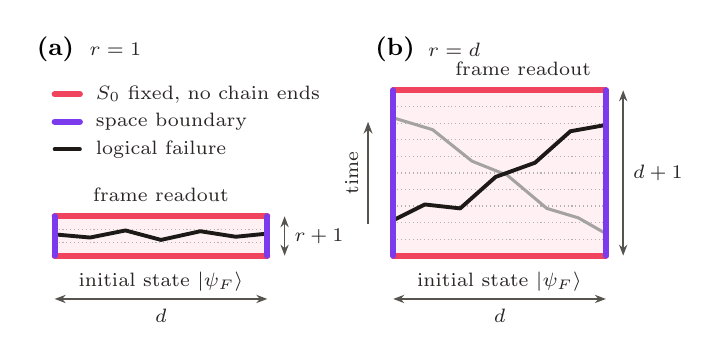
\begin{tikzpicture}[
  tb/.style={line width=2.2pt, draw=Szero, line cap=round},
  sb/.style={line width=2.2pt, draw=LogicalGold, line cap=round},
  layer/.style={line width=0.4pt, draw=InkSoft!45, densely dotted},
  chain/.style={line width=1.4pt, draw=ErrRed, line cap=round, line join=round},
  chain2/.style={line width=1.1pt, draw=ErrRed!40, line cap=round, line join=round},
  lab/.style={font=\scriptsize, text=InkDark},
]
\def\W{2.7}
% ---------------------------------------------------------------- panel (a): r = 1
\begin{scope}[shift={(0,0)}]
  \def\H{0.5}
  \node[font=\small\bfseries, anchor=west] at (-0.35,2.62) {(a)};
  \node[lab, anchor=west] at (0.32,2.62) {$r=1$};
  \fill[ClassB!12] (0,0) rectangle (\W,\H);
  \foreach \t in {0.167,0.333} {\draw[layer] (0,\t) -- (\W,\t);}
  \draw[chain] (0,0.27) -- (0.45,0.23) -- (0.9,0.32) -- (1.35,0.2) -- (1.85,0.31) -- (2.3,0.24) -- (\W,0.28);
  \draw[tb] (0,0) -- (\W,0);
  \draw[tb] (0,\H) -- (\W,\H);
  \draw[sb] (0,0) -- (0,\H);
  \draw[sb] (\W,0) -- (\W,\H);
  \node[lab, anchor=north] at (0.5*\W,-0.08) {initial state $\ket{\psi_F}$};
  \node[lab, anchor=south] at (0.5*\W,\H+0.06) {frame readout};
  \draw[{Stealth[length=1.4mm]}-{Stealth[length=1.4mm]}, line width=0.5pt, draw=InkSoft] (\W+0.22,0) -- node[right, lab] {$r+1$} (\W+0.22,\H);
  \draw[{Stealth[length=1.4mm]}-{Stealth[length=1.4mm]}, line width=0.5pt, draw=InkSoft] (0,-0.55) -- node[below, lab] {$d$} (\W,-0.55);
  % legend
  \draw[tb] (0,2.05) -- (0.32,2.05); \node[lab, anchor=west] at (0.4,2.05) {$S_0$ fixed, no chain ends};
  \draw[sb] (0,1.7) -- (0.32,1.7); \node[lab, anchor=west] at (0.4,1.7) {space boundary};
  \draw[chain] (0,1.35) -- (0.32,1.35); \node[lab, anchor=west] at (0.4,1.35) {logical failure};
\end{scope}
% ---------------------------------------------------------------- panel (b): r = d
\begin{scope}[shift={(4.3,0)}]
  \def\H{2.1}
  \node[font=\small\bfseries, anchor=west] at (-0.35,2.62) {(b)};
  \node[lab, anchor=west] at (0.32,2.62) {$r=d$};
  \fill[ClassB!12] (0,0) rectangle (\W,\H);
  \foreach \t in {0.21,0.42,...,1.95} {\draw[layer] (0,\t) -- (\W,\t);}
  \draw[chain2] (0,1.75) -- (0.5,1.6) -- (1.0,1.2) -- (1.45,1.02) -- (1.95,0.6) -- (2.35,0.48) -- (\W,0.28);
  \draw[chain] (0,0.45) -- (0.4,0.65) -- (0.85,0.6) -- (1.3,1.0) -- (1.8,1.18) -- (2.25,1.58) -- (\W,1.66);
  \draw[tb] (0,0) -- (\W,0);
  \draw[tb] (0,\H) -- (\W,\H);
  \draw[sb] (0,0) -- (0,\H);
  \draw[sb] (\W,0) -- (\W,\H);
  \node[lab, anchor=north] at (0.5*\W,-0.08) {initial state $\ket{\psi_F}$};
  \node[lab, anchor=south] at (0.5*\W+0.3,\H+0.06) {frame readout};
  \draw[{Stealth[length=1.4mm]}-{Stealth[length=1.4mm]}, line width=0.5pt, draw=InkSoft] (\W+0.22,0) -- node[right, lab] {$d+1$} (\W+0.22,\H);
  \draw[{Stealth[length=1.4mm]}-{Stealth[length=1.4mm]}, line width=0.5pt, draw=InkSoft] (0,-0.55) -- node[below, lab] {$d$} (\W,-0.55);
  \draw[-{Stealth[length=1.5mm]}, line width=0.6pt, draw=InkSoft] (-0.32,0.4) -- node[left, lab, rotate=90, anchor=south] {time} (-0.32,1.7);
\end{scope}
\end{tikzpicture}

\end{document}
